
% \harry{https://nbviewer.jupyter.org/github/amzn/emukit/blob/master/notebooks/Emukit-tutorial-experimental-design-introduction.ipynb}

% In machine learning, supervised problems are those for which we learn an input-output mapping by fitting some model to a dataset of input-output examples \cite{SupervisedLearning2020}. In many cases, we do not have access to such a dataset, however, we may have the ability to collect input-output pairs on-the-fly. This is the setting where active learning, and indeed experimental design, excel. They use heuristics to guide their choice of input points to evaluate, in the hopes of learning as much as possible about the underlying function, thus enabling us to create an accurate surrogate model of said function. In the context of experimental design, these heuristics are known as acquisitions functions, and in the case where the underlying function is a simulator, we say that the learned surrogate model is an \textit{emulator} if this model also reports how confident it is in its prediction (which is the case for GPs).
%  \harry{is this last sentence true? idk if the defn.is that formal}\matteo{I would drop the last part about reported confidence}

% \subsection{Acquisition Functions}

% Since the purpose of experimental design is to learn as much as possible about the underlying function, we would like an acquisition function that picks points that tell us as much as possible. We experimented with both uncertainty sampling (aka model variance), and integrated variance reduction. Both methods rely on being able to evaluate the predictive variance of our model with respect to any particular input; since GPs report this with each evaluation, they are a natural model choice for both uncertainty sampling and integrated variance reduction. Also, both methods rely on gradient-based optimizers to find the next point in the domain for which the respective measure is either maximised (in the case of uncertainty sampling) or minimized (in the case of integrated variance reduction) \cite{EmukitExperimentalDesign2020}.


% Uncertainty sampling \cite{lewisHeterogeneousUncertaintySampling1994}, selects points for which the current emulator prediction has high variance, with the rationale being that points with high variance are `interesting' and have more to be learned from than points we're already confident about. More formally, we wish to find points $\mathbf{x}$ at which the predictive variance $\sigma^{2}(\mathbf{x})$ of our model is maximal. In theory, high-variance regions of your learned function will be sampled frequently and therefore have their variance reduced. This should drive us to explore different points in the input domain which have greater predictive variance.
We performed experimental design with both uncertainty sampling (aka model variance) and integrated variance reduction. We found that uncertainty sampling was prone to a sort of `reward hacking' \cite{hadfield-menellInverseRewardDesign2020}. Our optimization continually collapsed to finding a configuration of 4/5 input parameters that produced extremely high variance when varying the remaining 1/5 parameter (`edgeLength', the length of roads between intersections, was this parameter). This meant that it failed to learn an accurate model of the underlying function, instead learning only about that one parameter. We originally attributed these highly variable outputs to a bug in our underlying simulation, which the experimental design process had learned to exploit. However, even after fixing this, uncertainty sampling still favoured extreme points in the input domain. This makes sense since the point of uncertainty sampling is to find points with high variance, however, this was not ideal for us; we wanted confident predictions across the full input domain, not just at the extremes.

Integrated variance reduction (IVR) \cite{sacksDesignAnalysisComputer1989} proved to be more effective for our purposes. We found that IVR was less prone to `reward hacking', and explored the parameter space more completely - this is reflected in our results.

% This acquisition function lets us finds points in the input domain which reduce the total variance of the model, where the total variance is computed using Monte-Carlo integration over some fixed number of randomly sampled points $\mathbb{X}$, given a prospective input point $\mathbf{x}$. The Monte-Carlo approximation takes following form \cite{EmukitExperimentalDesign2020}. \harry{This is copied https://mlatcl.github.io/mlphysical/lectures/04-02-emukit-and-experimental-design.html - is this acceptable w/ citation?}\nicholas{Probably not. Though there should be citations at the bottom of the page}


% \begin{equation}
% \begin{aligned}
% a_{I V R} &=
% & \approx \frac{1}{\# \text { samples }} \sum_{i}^{\text {# } \operatorname{samples}}\left[\sigma^{2}\left(\mathbf{x}_{i}\right)-\sigma^{2}\left(\mathbf{x}_{i} ; \mathbf{x}\right)\right]
% \end{aligned}
% \end{equation}

% Reiterating, prospective points $\mathbf{x}$ are computed by performing gradient descent to minimise $a_{I V R}$. We found that IVR was less prone to `reward hacking', and explored the parameter space more completely. % - this is reflected in our results.

\subsection{Experimental Design Results}


% \harry{permutations: Model\_variance timeloss, model\_variance co2, thompson sampling timeloss, thompson sampling co2 }

To assess the efficacy of our learned emulators, and experimental design in general, we performed t-tests in which we compared emulators learned using principled acquisition functions (uncertainty sampling and integrated variance reduction) to emulators learned using randomly sampled points. To do this, we first collected two sets of randomly sampled points using Emukit's `RandomDesign' utility; an initialization set of 20 points to initialize each GP with, and a test set of 100 points to evaluate the mean squared error of our models against. Then, we trained three emulators; one using uncertainty sampling (model\_variance) as our acquisition function, one using integrated variance reduction, and one using randomly sampled points. Every 50 iterations we evaluated each model on our test set - these results are plotted in Figure~\ref{fig:exp-design-loss}, please note that y-axes are on different scales. 

After all models had `seen' 500 points, we computed for each a final root mean squared error. Our results are summarised thus:

\begin{itemize}
    \item Integrated Variance Reduction was 13.98\% better than training on randomly sampled points when modelling CO2 per second.
    \item Integrated Variance Reduction was 7.63\% better than training on randomly sampled points when modelling time loss per second.
    \item Uncertainty Sampling was -8.25\% worse than training on randomly sampled points when modelling CO2 per second.
    \item Uncertainty Sampling was 2.58\% better than training on randomly sampled points when modelling time loss per second.
\end{itemize}

\begin{figure}[b!]
    \centering
    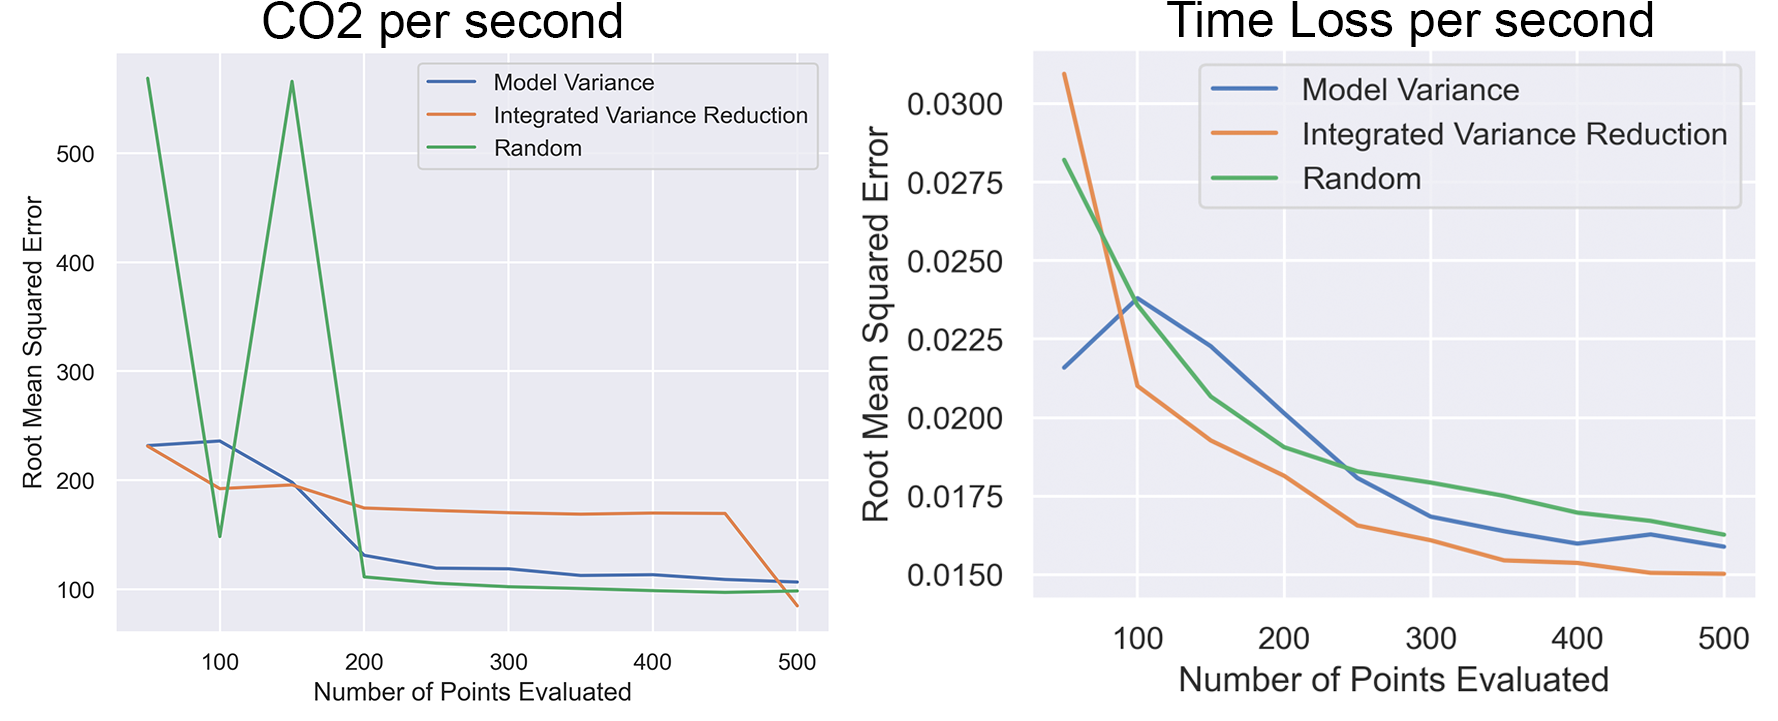
\includegraphics[width=0.9\textwidth]{images/exp_design_graph.png}
    \caption{Experimental Design results - root mean square error for models trained on intervals of 50 points acquired through uncertainty sampling (model variance), integrated variance reduction, and random sampling.}
    \label{fig:exp-design-loss}
\end{figure}

These results show that acquisition through integrated variance analysis is beneficial for our particular problem, however, acquisition through uncertainty sampling is less effective. The advantage of both acquisition functions diminishes relative to random sampling as more and more points are collected, implying that these techniques excel in settings where we have few input points. We ran experimental design 5 times for both CO2 and TimeLoss, then chose the lowest RMSE emulators to pass onto Bayesian Optimization. 
% All 5 runs produced similar RMSE models.